\documentclass{beamer}

\usepackage[utf8]{inputenc}
\usepackage{polski}
\usepackage{hyperref}
\usepackage{csquotes}
\usepackage{framed, color}
\usepackage{listings}
\usepackage{tikz}

\definecolor{shadecolor}{RGB}{192, 192, 192}
\definecolor{Gray}{RGB}{64,64,64}
\definecolor{White}{RGB}{255,255,255}

\lstloadlanguages{Java}
\definecolor{mygreen}{rgb}{0,0.6,0}
\definecolor{mygray}{rgb}{0.5,0.5,0.5}
\def\checkmark{\tikz\fill[scale=0.4](0,.35) -- (.25,0) -- (1,.7) -- (.25,.15) -- cycle;} 

\lstset{ 
  backgroundcolor=\color{white},   % choose the background color; you must add \usepackage{color} or \usepackage{xcolor}; should come as last argument
  basicstyle=\footnotesize,        % the size of the fonts that are used for the code
  breakatwhitespace=false,         % sets if automatic breaks should only happen at whitespace
  breaklines=true,                 % sets automatic line breaking
  captionpos=b,                    % sets the caption-position to bottom
  commentstyle=\color{mygreen},    % comment style
  deletekeywords={},            % if you want to delete keywords from the given language
  escapeinside={\%*}{*)},          % if you want to add LaTeX within your code
  extendedchars=true,              % lets you use non-ASCII characters; for 8-bits encodings only, does not work with UTF-8
  firstnumber=1,                % start line enumeration with line 1000
  frame=none,	                   % adds a frame around the code
  keepspaces=true,                 % keeps spaces in text, useful for keeping indentation of code (possibly needs columns=flexible)
  %keywordstyle=\color{blue},       % keyword style
  language=Java,                 % the language of the code
  morekeywords={ enum },            % if you want to add more keywords to the set
  numbers=left,                    % where to put the line-numbers; possible values are (none, left, right)
  numbersep=5pt,                   % how far the line-numbers are from the code
  numberstyle=\tiny\color{mygray}, % the style that is used for the line-numbers
  rulecolor=\color{black},         % if not set, the frame-color may be changed on line-breaks within not-black text (e.g. comments (green here))
  showspaces=false,                % show spaces everywhere adding particular underscores; it overrides 'showstringspaces'
  showstringspaces=false,          % underline spaces within strings only
  showtabs=false,                  % show tabs within strings adding particular underscores
  stepnumber=1,                    % the step between two line-numbers. If it's 1, each line will be numbered
  tabsize=2,	                   % sets default tabsize to 2 spaces
  title=\lstname                   % show the filename of files included with \lstinputlisting; also try caption instead of title
}

\setbeamercolor{frametitle}{bg=Gray, fg=White}

\newcommand{\slideTitle}
{
	\frametitle{
		\small{
			\textbf{Talk started. Talk ended. New tool added to the toolbox.}
			}
		}
}

\newcommand{\source}[2]{
    \begin{flushright}
        \hfill {\scriptsize \href{#1}{#2}}
    \end{flushright}
}

\begin{document}

\centering

% -----------------------

\begin{frame}
\frametitle{\textbf{}}

    \fbox{\begin{minipage}{33mm}
        \textbf{\Large{ Talk started}}
    \end{minipage}}
    \vskip 3mm
    \fbox{\begin{minipage}{3cm}
        \textbf{\Large{  Talk ended}}
    \end{minipage}}
    \vskip 3mm
    \fbox{\begin{minipage}{73mm}
        \textbf{\Large{New tool added to the toolbox}}
    \end{minipage}}

\end{frame}

% -----------------------

\begin{frame}
    \frametitle{\textbf{}}
    
    \textbf{
        \Large{What the hell Event Sourcing (ES) is and what that changes in my life?}
    }
    
\end{frame}

% -----------------------

\begin{frame}

    \frametitle{\textbf{}}
    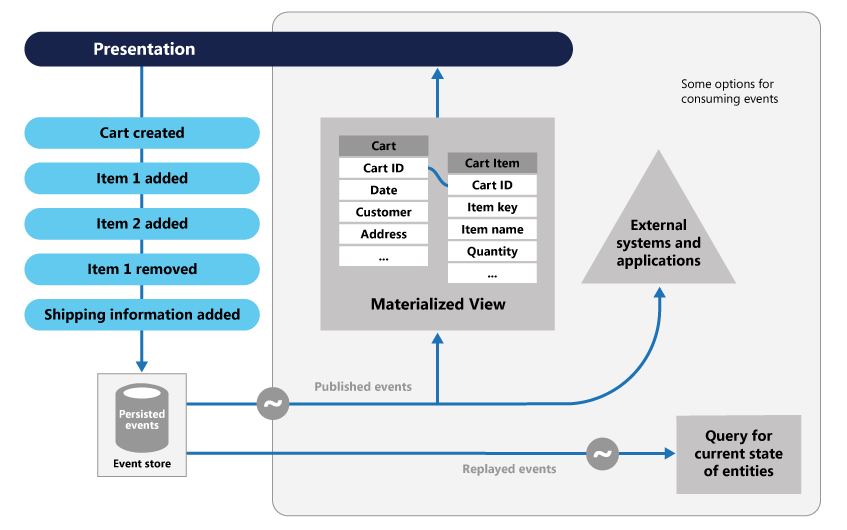
\includegraphics[height=65mm]{es_basic.png}
    \source{https://docs.microsoft.com/pl-pl/azure/architecture/patterns/event-sourcing}{Docs Microsoft}

\end{frame}

% -----------------------

\begin{frame}

    \frametitle{\textbf{}}
    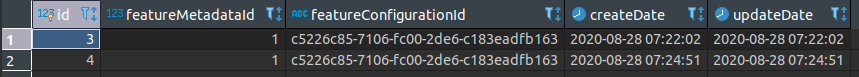
\includegraphics[width=\textwidth]{table.png}

\end{frame}

% -----------------------

\begin{frame}

    \frametitle{\textbf{}}
    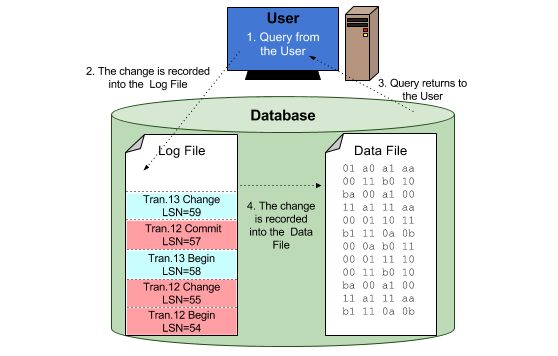
\includegraphics[height=65mm]{transaction_log.png}
    \source{https://sqlbak.com/academy/transaction-log}{source}
    
\end{frame}

\begin{frame}

    \frametitle{\textbf{}}
    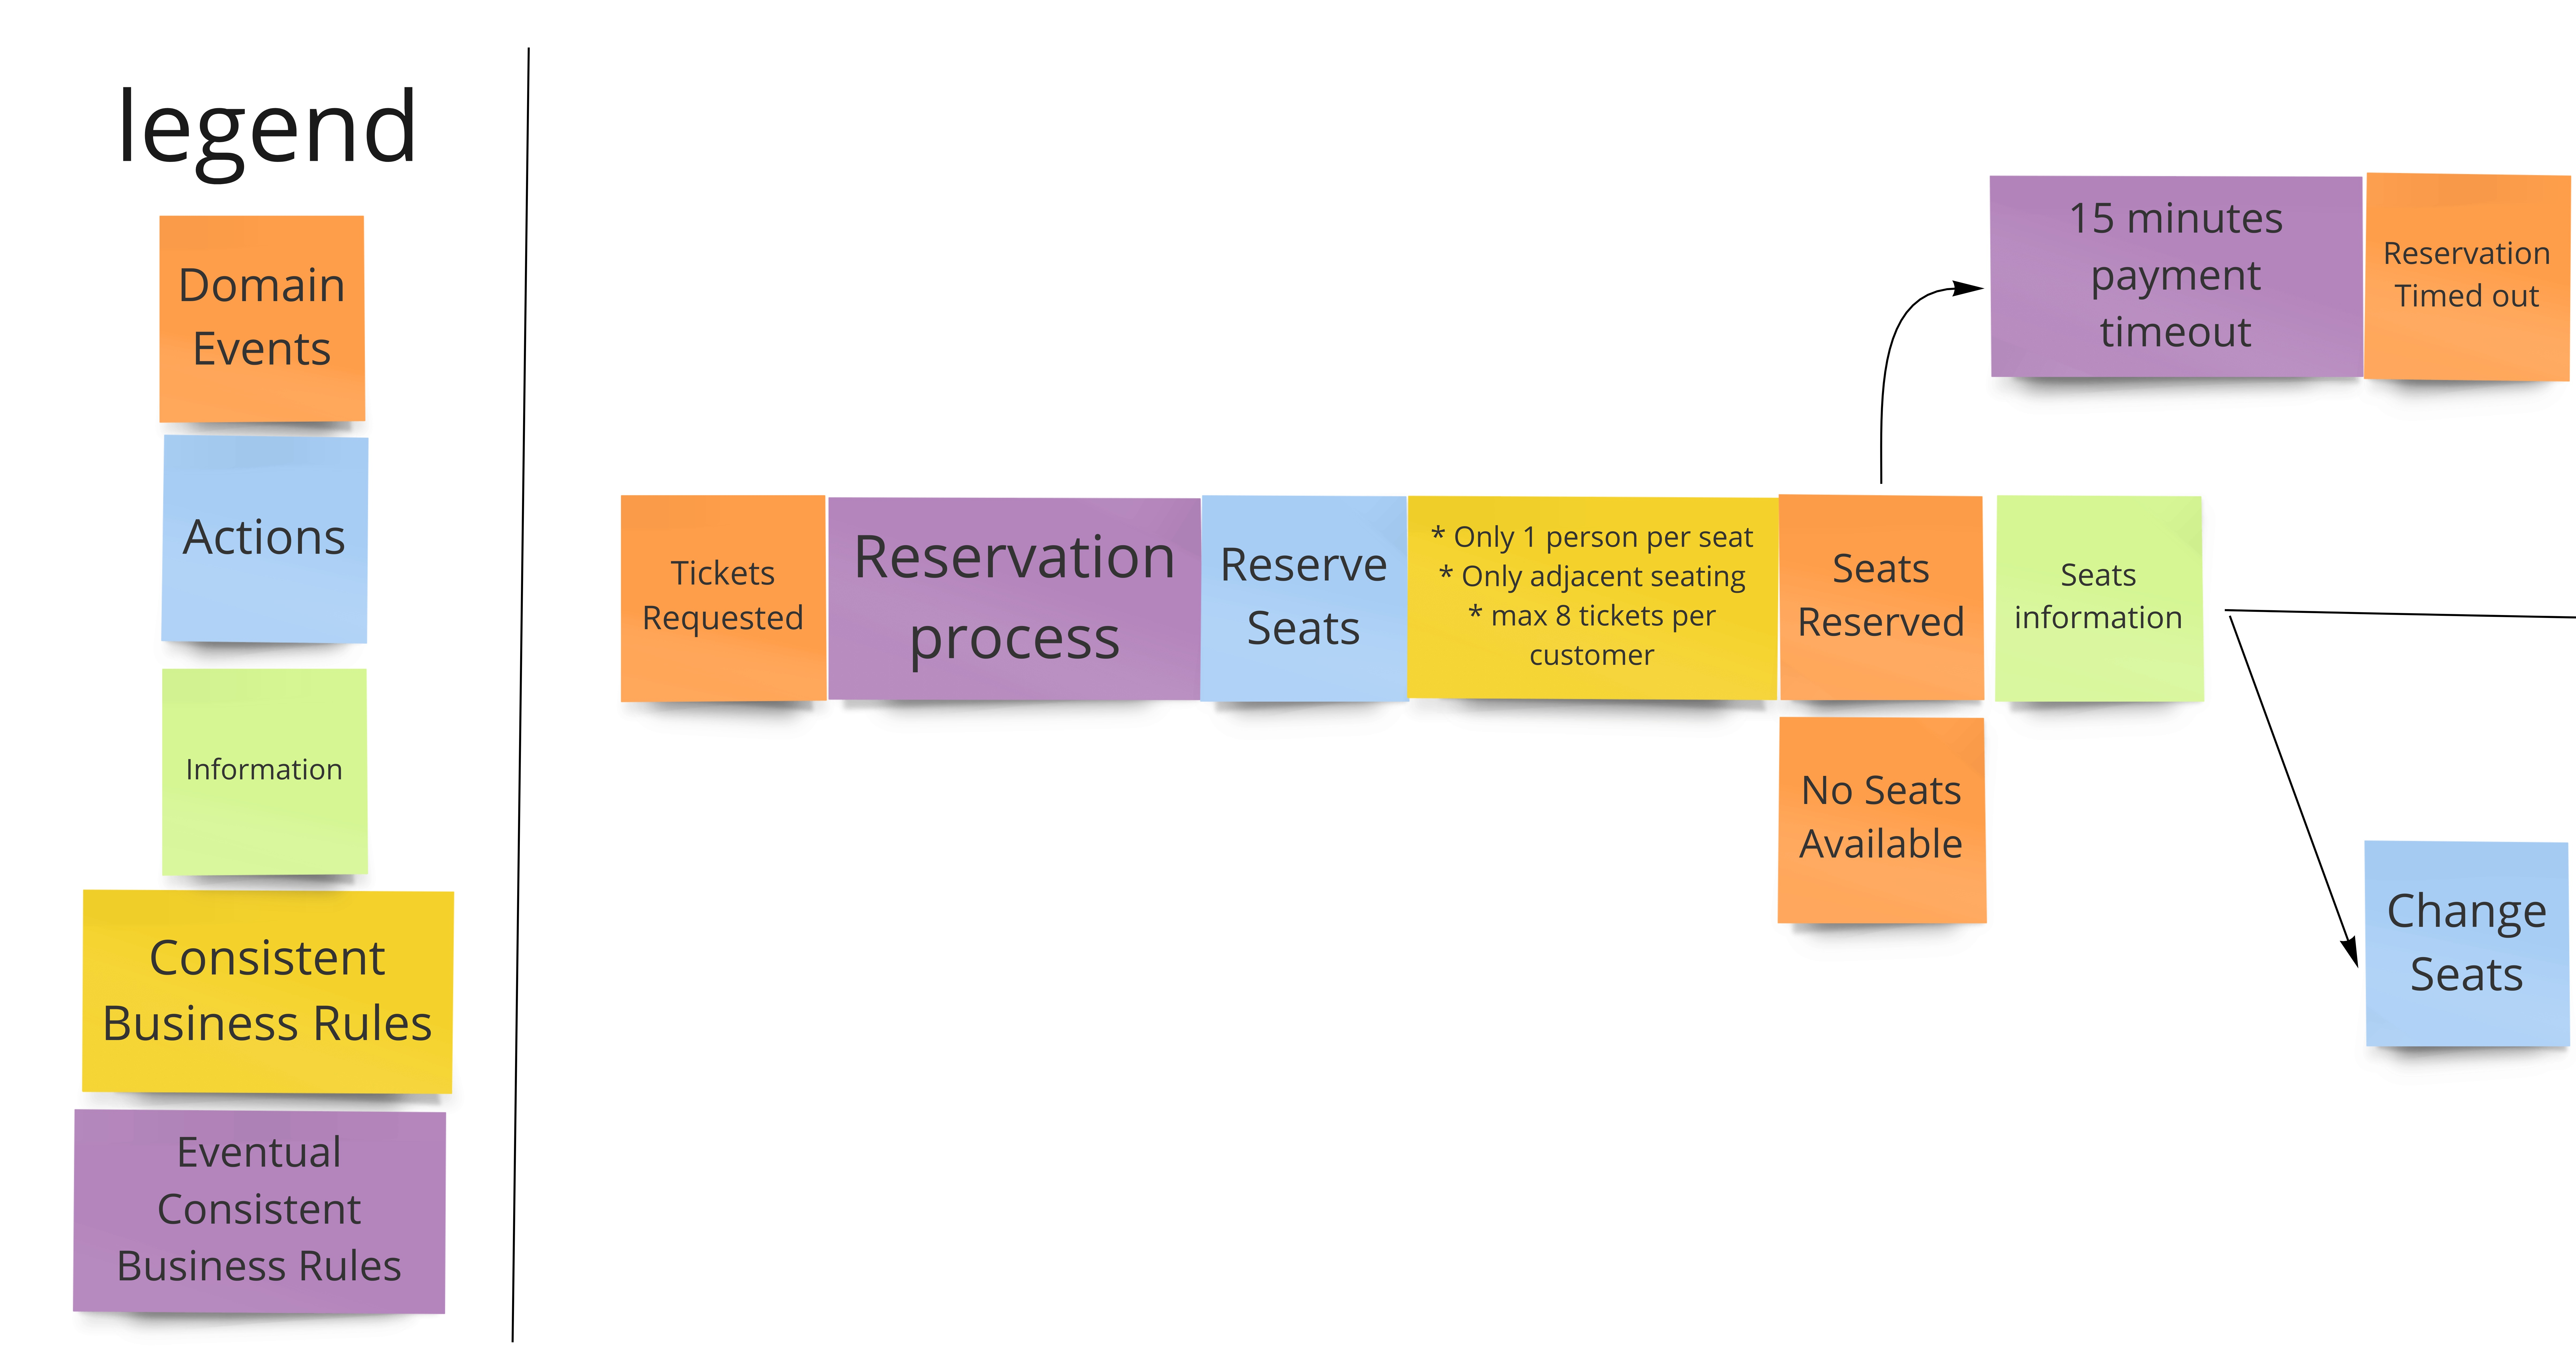
\includegraphics[width=\textwidth]{eventstroming.jpg}
    \source{https://baasie.com/2018/10/22/eventstorming-and-how-to-monitor-domain-events-for-product-management/}{source}
    
\end{frame}


% -----------------------

\begin{frame}

    \frametitle{\textbf{The most important rule}}

    \textbf{\Huge{You can't change the Past!}}

\end{frame}


% -----------------------

\begin{frame}

    \frametitle{\textbf{Glossary}}
    \textbf{
        \Large{
        \begin{itemize}
            \item Event
            \item Event Store
            \item Event Stream
            \item Projection
            \item Snapshot
        \end{itemize}
        }
    }

\end{frame}

% -----------------------

\begin{frame}

    \textbf{\Huge{Let's take a look into the code}}

\end{frame}

% -----------------------

\begin{frame}

    \textbf{\Huge{"Versioning in an Event Sourced System"}}
    
    \vskip 15mm

    \source{https://dddeurope.com/2017/speakers/greg-young/}{\Large{Gregory Young}}

\end{frame}

% -----------------------

\begin{frame}

    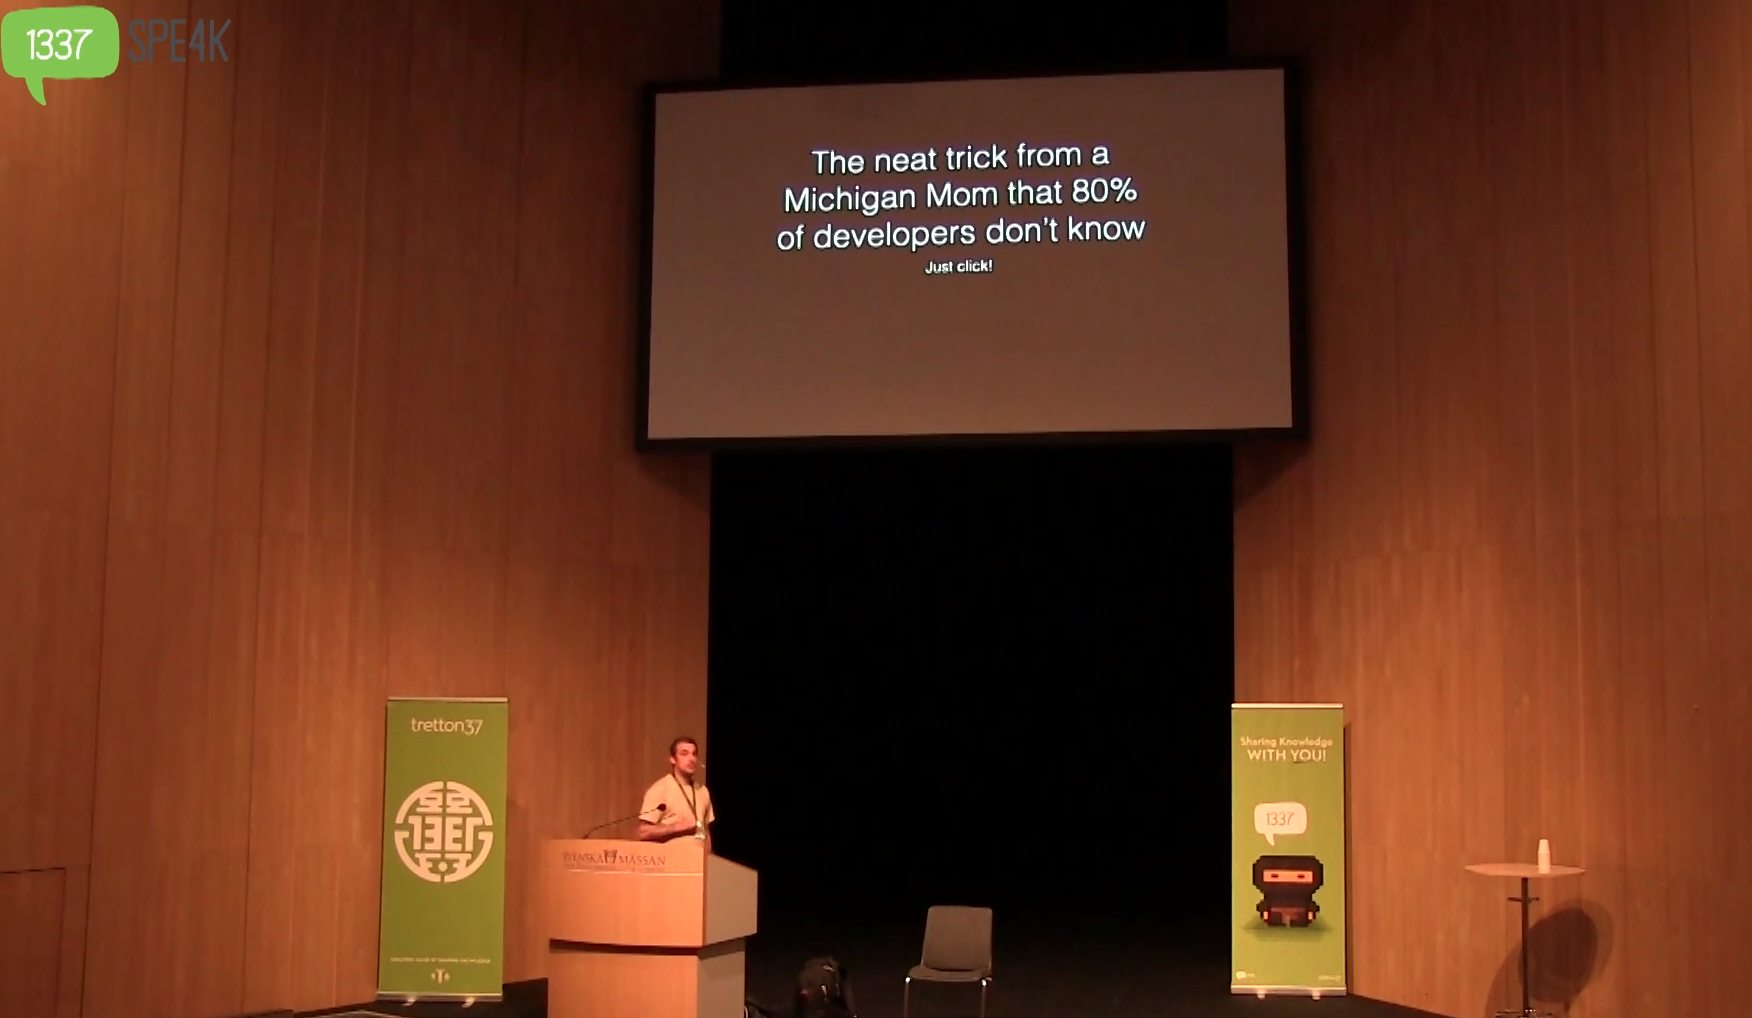
\includegraphics[width=\textwidth]{greg_young.png}
    \source{https://vimeo.com/108441214}{\Large{The art of destroying software}}

\end{frame}

% -----------------------

\begin{frame}

    \frametitle{\textbf{Lesson learned}}
    \textbf{
        \large{
        \begin{itemize}
            \item Weak schema
            \item Event versioning
            \item Saving all stack
            \item Snapshots
            \item Avoid "and"
            \item Errors
            \begin{itemize}
                \item compensation action
                \item deleting a stream is ok
                \item copy and replace
            \end{itemize}
            \item public/private streams
            \item two aggregates one stream
            \item one aggregate two streams
            \item copy and transform $\rightarrow $ migrations
        \end{itemize}
        }
    }

\end{frame}

\begin{frame}[fragile]

    \frametitle{\textbf{Weak schema}}
    \begin{lstlisting}
        {
            "id": 1,
            "firstName": "John"
            "lastName" : "Smith",
            "age" : 25
        }\end{lstlisting}
    \begin{lstlisting}[language=Java]
        public class Client
        {
            public int Id { get; set; }
            public string FirstName { get; set; }
            public string LastName { get; set; }
            public int Age { get; set; }
        }\end{lstlisting}

\end{frame}

\begin{frame}

    \frametitle{\textbf{Weak schema}}
    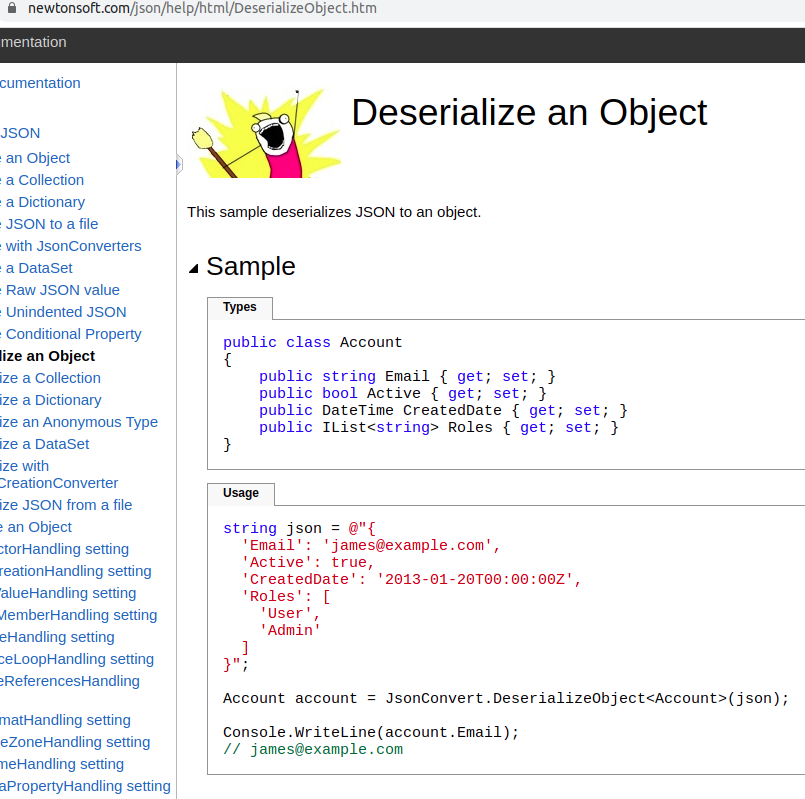
\includegraphics[height=8cm]{newtonsoft.png}

\end{frame}

\begin{frame}[fragile]

    \frametitle{\textbf{Weak schema}}

    \begin{flushleft}
        \textbf{\LARGE{Mapping}}
        \vskip 1mm
        \begin{lstlisting}
            Map.To<Client>()
                .WhenAbsent("age", -99)
                .WhenAbsentError("id")\end{lstlisting}

        \textbf{\LARGE{Wrapping}}
        \vskip 1mm
        \begin{lstlisting}[basicstyle=\scriptsize]
    public class ClientWrapper {
        private readonly JObject _json;

        public ClientWrapper(string json) {
            _json = JObject.Parse(json);
        }

        public Guid Id {
            get { return Guid.Parse(_json["id"]); }
            set { _json["id"] = value.ToString(); }
        }
        (...)
    }\end{lstlisting}
    \end{flushleft}

\end{frame}

\begin{frame}[fragile]

    \frametitle{\textbf{Event versioning}}
    \begin{itemize}
        \item Double publish (v1, v2)
        \item Constructor with previous version
    \end{itemize}
    \vskip 3mm
    \begin{flushleft}
        \textbf{Example}
    \end{flushleft}
    
    \begin{lstlisting}
    ClientCreated_v2 ConvertFrom(ClientCreated_v1 e) {
        return new ClientCreated_v2(e.Id, -99);
    }

    ClientCreated_v1 ConvertFrom(ClientCreated_v2 e) {
        return new ClientCreated_v1(e.Id);
    }\end{lstlisting}

\end{frame}

\begin{frame}[fragile]

    \frametitle{\textbf{Sabing all stack}}
    \begin{lstlisting}
    public void Apply(ItemSold e) {
        _tax = e.Subtotal * .22;
    }\end{lstlisting}

\end{frame}

\begin{frame}[fragile]

    \frametitle{\textbf{Sabing all stack}}
    \begin{lstlisting}
    public void Apply(ItemSold e) {
        if(e.Date < Convert.ToDateTime("1/1/2017")) {
            _tax = e.Subtotal * .22;
        } else {
            _tax = e.Subtotal * .23;
        }
    }\end{lstlisting}

\end{frame}

\begin{frame}[fragile]

    \frametitle{\textbf{Sabing all stack}}
    \begin{lstlisting}
public void SellItem(...) {
    //snip
    var tax = subtotal * .23;
    Apply(new ItemSold(_id,....,tax));
}

public void SellItem(...) {
    //snip
    var customerScore = _externalService
                    .GetCustomerScoreFor(customer);

    Apply(new ItemSold(_id,....,customerScore));
}\end{lstlisting}

\end{frame}

\begin{frame}

    \frametitle{\textbf{Lesson learned}}
    \textbf{
        \large{
        \begin{itemize}
            \item Weak schema \checkmark
            \item Event versioning \checkmark
            \item Saving all stack \checkmark
            \item Snapshots
            \item Avoid "and"
            \item Errors
            \begin{itemize}
                \item compensation action
                \item deleting a stream is ok
                \item copy and replace
            \end{itemize}
            \item public/private streams
            \item two aggregates one stream
            \item one aggregate two streams
            \item copy and transform $\rightarrow $ migrations
        \end{itemize}
        }
    }

\end{frame}

\end{document}